\documentclass[a4paper]{article}

\usepackage[utf8]{inputenc}
\usepackage[T1]{fontenc,url}
\usepackage{cite}
\usepackage{hyperref}
\usepackage{amsmath, amssymb}
\usepackage{tikz}
\usepackage{graphicx}
\usepackage{parskip}
\usepackage{lmodern}
\usepackage{algorithm}
\usepackage{algpseudocode}
\usepackage{epigraph}
\usepackage{listings}
\usepackage{float}
\usepackage{subcaption}

\begin{document}
\title{FYS-STK4155 -- Project 2}
\author{Jing Sun and Endrias Getachew Asgedom}

\maketitle
\begin{abstract}
We investigate regression and classification problems using a noise contaminated Franke function and the MNIST dataset. To solve the regression problem, we use a fully connected neural network (NN) and Stochastic Gradient Descent (SGD)-based Ordinary Least Square (OLS) and Ridge regression methods. For the linear regression methods, we first tune the learning rate $\eta$ using the Gradient descent (GD) method and perform a grid search with a $5$-fold cross validation to find the optimal hyperparameters of the SGD algorithm. Similarly, for the NN approach, we tune the hyperparameters with a grid search and manually adjust the activation functions, the number of hidden layers, and the number of neurons. The performances of the SGD-based OLS and Ridge regression methods are almost equivalent, but slightly worse compared to their corresponding analytical inversion-based methods. Furthermore, linearly decaying the learning rate as a function of the number of epochs results in the most stable and accurate prediction with an $R^2$-score of $0.743$ and mean square error (MSE) of $0.020$. Nevertheless, a two-hidden-layer NN with the Leaky ReLU activation function performs also well but slightly worse than the corresponding linear regression methods with an $R^2$-score of $0.692$ and MSE of $0.024$. However, the same structure NN implemented by using the $\mathbf{Scikit}$-$\mathbf{learn}$ library produces the best result of all with an $R^2$-score of $0.841$ and an MSE of $0.013$. To classify the handwritten digits in the MNIST dataset, we use the multinomial logistic (softmax) regression and a fully connected NN. Both the methods use the cross-entropy function as the cost function and the SGD algorithm to find the optimal weights and biases. The test accuracy for a single-hidden-layer NN with $50$ neurons is $0.961$ while for the softmax regression it is $0.958$. A similar implementation using $\mathbf{Scikit}$-$\mathbf{learn}$ library produces a test accuracy of $0.969$ for both the NN approach and the softmax regression.
\noindent
\end{abstract}
\newpage

\tableofcontents

\begin{center}
    GitHub repository at \url{https://github.com/endrias34/FYS-STK4155/tree/master/Project-2}
\end{center}

\newpage

%%% MACROS
\newcommand{\half}{\frac{1}{2}}
\newcommand{\dx}{{\Delta x}}
\newcommand{\bigO}{{\mathcal{O}}}

\section{Introduction}
Machine Learning (ML) applications can be either supervised where prior knowledge of the system is known or unsupervised (e.g. “learning without a teacher”) \cite{hastie}. The latter approach aims to identify patterns and relationship in data sets without any prior knowledge. In supervised learning, a set of training data consisting of input data and the corresponding output data representing the ground truth are provided. The essence of supervised learning is to extract important correlations about the physical processes characterizing the given examples and then perform predictions on the future (unseen) data. 

In this project, we study the two main types of problems that often arise in supervised learning applications. These problems are: regression and classification. The algorithms used here to solve such types of problems are neural networks (NNs), linear regression, and multinomial logistic regression methods. NNs have recently received a great deal of attention in various fields of sciences and engineering following its successful applications within fields such as image recognition and natural language processing. In addition, easier access to affordable and powerful hardware (CPU and GPU) solutions together with user-friendly open-source software has been the key to the accelerated use of NNs for handling big data within various areas of technology. 

Finding the values of the parameters that minimize the cost function is a key task for all supervised learning applications. Thus, in this project, we utilize the Gradient Descent (GD) and the Stochastic Gradient Descent (SGD), with minibatches, algorithms to find the optimal model parameters. The first part of this project is an extension to the linear regression investigation we did in project 1 \cite{Jing2020}. We use the same dataset as in project 1, the noisy Franke function, but perform the ordinary least square (OLS) and Ridge regressions using SGD. To tune the learning rate, the GD method is used and the optimal hyperparameters are estimated using a grid search with a $5$-fold cross validation. Next, we perform regression using NNs and similarly estimate the hyperparameters using a grid search with a $5$-fold cross validation. To benchmark our implementation of the NNs, we compare our results with the results of $\mathbf{Scikit}$-$\mathbf{learn}$. The last section of this project analyses the problem of classification using the MNIST (Modified National Institute of Standards and Technology) dataset. We use the multinomial logistic regression and a NN to classify the handwritten digits. The performances of the two methods are analysed quantitatively and compared with the corresponding implementation of the $\mathbf{Scikit}$-$\mathbf{learn}$ library.

\section{Theory}
In this section, a brief description of the methods adopted in this project are given, starting with an introduction to the theory of the SGD algorithm. In the following subsections, the basic concepts of (binary and multinomial) logistic regression and NNs will be discussed.

\subsection{Stochastic Gradient Descent}
The basic components of a ML task are observations $\mathbf{x}$ which is a set of data, a model which describes a functional relationship between the observations and the goal of the task by a set of parameters $\boldsymbol{\beta}$, and a cost function $\mathcal{C}$ which provides a way to judge how well the model explains the observations. The point of fitting the model is to find the values of the parameters that minimize the cost function. Thus, the minimization problem is always a key issue of a ML task \cite{Pankaj}. In this section, we introduce the GD and the SGD, with minibatches, algorithms which are the most powerful and widely used methods for performing the minimization of the cost function.

In the GD algorithm, the parameters $\boldsymbol{\beta}$ are iteratively adjusted in the direction of the negative value of the gradient for a given number of epochs or until it reaches a given tolerance, which can be expressed as
\begin{align}
    v_{t} &= \eta_t \nabla_\beta \mathcal{C}(\beta_t) \nonumber \\
    \beta_{t+1} &= \beta_t - v_{t},
\end{align}
where $\nabla_\beta \mathcal{C}(\boldsymbol{\beta})$ is the gradient of $\mathcal{C}(\boldsymbol{\beta})$ with respect to $\boldsymbol{\beta}$ and $\eta_t$ is the learning rate, which is a hyperparameter that controls how big a step we should take in the direction of the gradient at time step $t$ \cite{Pankaj}. For smaller values of $\eta$, the method takes longer time to converge and might fall inside a local minimum. For larger values of $\eta$, the method might be more unstable and struggle with convergence because it might pass the minimum altogether and diverge. In general, it is always computationally heavy to calculate the gradient on the entire dataset, which is especially a problem when handling large amounts of data. Besides, there is a problem of a local minimum being misinterpreted as the global minimum. 

The SGD algorithm is a generalization of the GD algorithm which can alleviate the above mentioned problems. Instead of calculating the actual gradient over the entire dataset at each gradient descent step, we perform the GD method on randomly chosen minibatches. A minibatch is a subset of a fixed number of the entire dataset. Assuming there are $N$ samples in total and we set the mini-batch size as $M$, then there are $N/M$ minibatches. We use $B_k$ where $k=1,2,...,N/M$ to represent a single minibatch. We then cycle over all $k=1,2,...,N/M$ minibatches one at a time, and use the mini-batch approximation to the gradient to update the parameters $\boldsymbol{\beta}$ at every step $K$. A full iteration over all $N/M$ minibatches is called an epoch \cite{Pankaj}. Approximating the gradient using a single minibatch at each gradient step in the SGD method can be represented as
\begin{align}
    \nabla_\beta \mathcal{C}^{\textsc{MB}}(\beta) = \sum_{i \in B_k} \nabla_\beta c_i(x_i,\beta).
\end{align}
The SGD parameter update can be expressed as
\begin{align}
    v_{t} &= \eta_t \nabla_\beta \mathcal{C}^{\textsc{MB}}(\beta)\nonumber \\
    \beta_{t+1} &= \beta_t - v_{t}.
\end{align}
The SGD algorithm can significantly speed up the calculation because it does not have to use the entire dataset to compute the gradient. In addition, the stochasticity can decrease the chance that our fitting algorithm gets stuck in isolated local minimum \cite{Pankaj}. 

\subsection{Logistic Regression}
A linear regression analysis can be used to find a functional relationship describing how a set of continuous variables vary based on some independent variables. However, the outcomes of classification problems are discrete variables (i.e. categories). For such cases, we represent the design matrix of the input data as $\mathbf{X}\in\mathbb{R}^{N\times P}$ which is made of $N$ samples and each sample has $P$ features. A classification problem has a set of discrete dependent variables ${y}^{(i)}$ with values in the range of $k=0,1,...,K-1$ which enumerate the $K$ classes. To solve such a problem, the linear regression methods become not optimal. Therefore, we introduce logistic regression in this section. Logistic Regression is a fundamental ML technique that uses a linear weighted combination of features and generates probability-based predictions of different classes \cite{CNTKB}. 

The simplest classification problem is when there are only two classes, which is called a binary logistic regression problem. For binary logistic regression, there are only two possible outcomes of the regression $y^{(i)} \in \{0, 1\}$. The logistic function here is also called the sigmoid function. It is defined as
\begin{align}
    \sigma_\beta(x) 
    = \frac{1}{1+\mathrm \exp{(-{\beta}^{\top} x)}}
    = \frac {\exp{({\beta}^{\top} x)}}{1+\mathrm \exp{({\beta}^{\top} x)}}.
\end{align}
Note that $1-\sigma_\beta(x)= \sigma_\beta(-x)$. The regression parameters $\boldsymbol{\beta}$ are trained to minimize the cost function \cite{softmax}
\begin{align}
    \mathcal{C}(\beta) = -\left[ \sum_{i=1}^N y^{(i)} \log \sigma_\beta(x^{(i)}) + (1-y^{(i)}) \log (1-\sigma_\beta(x^{(i)})) \right].
\end{align}
Since there are only two categories with the output of the logistic regression analysis $y^{(i)}$ either $0$ or $1$, a single parameter $\boldsymbol{\beta}$ is enough to predict the probabilities of the two classes as
\begin{align}
    &\mathbf{P}(y^{(i)}=1|x^{(i)};{\beta}) 
    = \frac{\exp{(\beta^{\top} x^{(i)})}}{1+ \exp{(\beta^{\top} x^{(i)})}},\nonumber\\
    &\mathbf{P}(y^{(i)}=0|x^{(i)};{\beta}) 
    = 1 - \mathbf{P}(y^{(i)}=1|x^{(i)};{\beta}) .
\end{align} 
Multinomial logistic regression is a more complicated classification method that generalizes logistic regression to multiclass problems, i.e. the regression has multiple possible outputs and each of them represents a single class. The softmax function is a generalization of the sigmoid function to handle this kind of cases with multiple classes. In the softmax regression setting, the label $y$ takes on $K$ different values rather than only two. For example, in the MNIST digit recognition task studied in this project, we have $y^{(i)} \in \{0, 1, \ldots, 9\}$ i.e. $K=10$ different classes.

The softmax function outputs a $K$-dimensional vector representing $K$ estimated probabilities for a given test input $x^{(i)}$. The summation of the $K$ estimated probabilities equals to 1 and the highest probability is then selected as the predicted label. It can be expressed as 
\begin{align}
    \sigma_\beta(x^{(i)}) =
    \begin{bmatrix}
    \mathbf{P}(y^{(i)} = 0 | x^{(i)}; {\beta}) \\
    \mathbf{P}(y^{(i)} = 1 | x^{(i)}; {\beta}) \\
    \vdots \\
    \mathbf{P}(y^{(i)} = K-1 | x^{(i)}; {\beta})
    \end{bmatrix}
    =
    \frac{1}{ \sum_{j=0}^{K-1} \exp{(\beta_j^{\top} x^{(i)}) }}
    \begin{bmatrix}
    \exp{(\beta_0^{\top} x^{(i)})} \\
    \exp{(\beta_1^{\top} x^{(i)})} \\
    \vdots \\
    \exp{(\beta_{K-1}^{\top} x^{(i)})} \\
    \end{bmatrix}
\end{align}
The cost function used for softmax regression is defined as
\begin{align}
    \mathcal{C}(\beta) = - \left[ \sum_{i=1}^{N} \sum_{k=0}^{K-1}  1\left\{y^{(i)} = k\right\} 
    \log \frac {\exp{(\beta_{k}^{\top} x^{(i)})}}{\sum_{j=0}^{K-1} \exp{(\beta_{j}^{\top} x^{(i)})}}\right],
    \label{mclog-cost}
\end{align}
where $1\{\cdot\}$ is the indicator function which means $1\{\hbox{a true statement}\}=1$ and $1\{\hbox{a false statement}\}=0$ \cite{softmax}. The cost function (also known as the cross-entropy function) can also be expressed as
\begin{align}
    \mathcal{C}(\beta) 
    = - \left[ \sum_{i=1}^N (1-y^{(i)}) \log (1-\sigma_\beta(x^{(i)})) + y^{(i)} \log \sigma_\beta(x^{(i)}) \right].
    \label{cost_softmax}
\end{align}
Note that in softmax regression, we have 
\begin{align}
    \mathbf{P}(y^{(i)} = k | x^{(i)};\beta) 
    = \frac{\exp(\beta_k^{\top} x^{(i)})}{\sum_{j=0}^{K-1} \exp(\beta_j^{\top} x^{(i)})}.
\end{align}

\subsection{Neural Networks}
\label{sec-nn}
As the name suggests, neural networks (NNs) are inspired by and partially modeled on biological neural networks wherein neurons interact by sending signals in the form of mathematical functions between layers \cite{lec}. Neurons are the most basic components and computational units of a NN. An arbitrary number of neurons form a layer.  Typically, the building blocks of a NN consist of an input layer, hidden layer(s) and an output layer. Such NNs are called multi-layer perceptrons (MLPs) which are what we use for both classification and regression in this project. Figure \ref{ANN} shows an example of a MLP with two hidden layers. The neurons of a NN are connected from the previous layer via matrix–vector multiplication and non-linear activation functions. They contain adaptive weight variables which can be tuned by a learning algorithm.

\begin{figure}[H]
  \centering
  \includegraphics[width=\columnwidth]{Project2/ANN.png}
  \caption{Example of a MLP with two hidden layers \cite{nielsenneural}.}
    \label{ANN}
\end{figure}

\subsubsection{Feed-forward}
Feed-forward means starting from the input layer and propagate to the output layer. The forward computation from one layer to the next is known as forward propagation. We denote the labeled training examples as $(x^{(i)}, y^{(i)})$ and the number of layers in the network as $L$. The weight associated with the connection between the $j^{th}$ neuron in the $l^{th}$ layer and $k^{th}$ neuron in the $(l-1)^{th}$ layer is represented as $W^{(l)}_{jk}$. The bias of the $j^{th}$ neuron in the $l^{th}$ layer is represented as $b^{(l)}_j$. 

As an example, we show how to feed-forward from the input layer to the first hidden layer. Assuming the input layer consists of $K$ neurons so that a single input vector can be represented as $x^{(i)}\in\mathbb{R}^{K \times 1}$. The input vectors are fed forward to all the $J$ neurons in the first hidden layer. The non-linear transform from the input layer to the first hidden layer can be mathematically expressed as
\begin{align}
    f^{(2)}(\mathbf{z}^{(2)}) 
    &= f^{(2)}\left(\left[\begin{array}{ccc}
        W^{(1)}_{11} &... &W^{(1)}_{1J} \\
        \vdots &  &\vdots\\
        W^{(1)}_{J1} &... &W^{(1)}_{JK} \\
        \end{array} \right] 
        \left[\begin{array}{c}
           x^{(1)}_{1} \\
           \vdots\\
           x^{(1)}_{K} \\
        \end{array}\right] + 
        \left[\begin{array}{c}
           b^{(1)}_{1} \\
           \vdots\\
           b^{(1)}_{J} \\
        \end{array}\right]\right)\nonumber\\
    &= f^{(2)}(\mathbf{W}^{(1)}\mathbf{x}^{(1)} + \mathbf{b}^{(1)}),
\label{f(z2)} 
\end{align}
where $f(\cdot)$ is the so-called activation function. Different layers can have different activation functions. The matrix $\mathbf{W}^{(1)} \in \mathbb{R}^{J \times K}$ represent the weights and $\mathbf{b} ^{(1)} \in \mathbb{R}^{J}$ represent the biases. We set $\mathbf{x}^{(1)} = \mathbf{a}^{(1)}$, equation \ref{f(z2)} can then be written as $\mathbf{a}^{(2)} = f^{(2)}(\mathbf{z}^{(2)})$, where $\mathbf{z}^{(2)} = \mathbf{W}^{(1)} \mathbf{a}^{(1)} + \mathbf{b}^{(1)}$. 

The activation for any neuron $j$ in any layer $l$ can be represented as 
\begin{align}
    z_j^{(l)}
    &= \sum_{k}^{ } W^{(l)}_{jk} a^{(l-1)}_k + b^{(l)}_j \nonumber \\
    a_j^{(l)} 
    &= f^{(l)}(z_j^{(l)}).
\end{align}
The general equations of the feed forward process of a NN can be further simplified as
\begin{align}
    \mathbf{z}^{(l)}
    = \mathbf{W}^{(l)}\mathbf{a}^{(l-1)} + \mathbf{b}^{(l)},
\label{_auto11} 
\end{align}
\begin{align}
    \mathbf{a}^{(l)}=f^{(l)}(\mathbf{z}^{(l)}).
\end{align}

\subsubsection{Back-propagation}
When the feed forward is completed, the error between the estimated value and the true value is calculated for updating the weights and biases through back-propogation \cite{lec} where we iterate backwards from the last layer to the first hidden layer. Backpropagation is about understanding how changing the weights and biases in a network changes the cost function, which ultimately allows us to compute the partial derivatives $\frac{\partial  \mathcal{C}}{\partial w^l_{jk}}$ and $\frac{\partial \mathcal{C}}{\partial b^l_j}$ \cite{nielsenneural}. Let $\mathcal{C}$ denote the cost function, the error of the output layer is represented as 
\begin{align}
    \delta_j^L= \frac{\partial \mathcal{C}}{\partial a_j^L} \odot f'(z_j^L)
    \label{delta_j^L}
\end{align}
where $\odot$ represents the hadamard product. The term $f'(z_j^L)$ measures how fast the activation function $f'$ is changing at $z_j^L$. The term $\frac{\partial \mathcal{C}}{\partial a_j^L}$ measures how fast the cost is changing as a function of the $j$th output activation \cite{nielsenneural}. Equation \ref{delta_j^L} can be rewritten as a matrix-vector form, as
\begin{align}
    \mathbf{\delta}^{L}= {\bigtriangledown}_{a} \mathcal{C} \odot f'(\mathbf{z}^L) ,
    \label{delta_j^L}
\end{align}
where ${\bigtriangledown}_{a} \mathcal{C}$ denotes a vector whose components are the partial derivatives $\frac{\partial \mathcal{C}}{\partial a_j^L}$. The general equation representing moving the error backward through the network from any layer $l+1$ to layer $l$ can be expressed as
\begin{align}
    \mathbf{\delta}^l = ((\mathbf{W}^{l+1})^T \mathbf{\delta}^{l+1}) \odot f'(\mathbf{z}^l),
\label{delta^l}
\end{align}
where $(\mathbf{W}^{(l+1)})^T$ is the transpose of the weight matrix $\mathbf{W}^{(l+1)}$ for the $(l+1)$th layer. The rate of change of the cost with respect to any bias in the network can be computed by 
\begin{align}
    \frac{\partial \mathcal{C}}{\partial b^l_j} = \delta^l_j.
    \label{delta_j^l}
\end{align}
Similarly, the rate of change of the cost with respect to any weight in the network can be computed by 
\begin{align}
    \frac{\partial \mathcal{C}}{\partial w^l_{jk}} = a_k^{l-1} \delta^l_j.
    \label{delta_j^l}
\end{align}
The back-propagation process is summarized in Algorithm \ref{alg-bac}.
\begin{algorithm}[H]
    \caption{Back-propagation}
    \label{alg-bac}
    \begin{algorithmic}
        \State 1. $\textbf{Input $\mathbf{x}$:}$ calculate the activation $\mathbf{a}^{1}$ for the input layer.
        \State 2. $\textbf{Feed-forward:}$ starting with the first layer, exploit the feed-forward architecture to compute $\mathbf{z}^{l}=\mathbf{W}^{l}\mathbf{a}^{l-1}+\mathbf{b}^{l}$ and $\mathbf{a}^{l}=f(\mathbf{z}^{l})$ for each subsequent layer $l=2,3,...,L$.
        \State 3. $\textbf{Error at the top layer:}$ compute the error of the top layer using $\mathbf{\delta}^{L}= {\bigtriangledown}_{a} \mathcal{C} \odot f'(\mathbf{z}^L)$.
        \State 4. $\textbf{Back-propagate the error:}$ propagate the errors backwards and compute $\mathbf{\delta}^l = ((\mathbf{W}^{l+1})^T \mathbf{\delta}^{l+1}) \odot f'(\mathbf{z}^l)$ for each layer $l=L-1,L-2,L-3,...,2$.
        \State 5. $\textbf{Calculate the gradient:}$ the gradient of the cost function is given by $\frac{\partial \mathcal{C}}{\partial w^l_{jk}} = a_k^{l-1} \delta^l_j$ and $\frac{\partial \mathcal{C}}{\partial b^l_j} = \delta^l_j$.
    \end{algorithmic}
\end{algorithm}

\subsubsection{Activation functions}
Activation functions are commonly adopted when deriving both forward and backward propagation algorithms. An activation function should meet certain properties. It should be differentiable (continuous), non-constant and reach saturation at both ends of the range. Besides, it should change quickly between the saturation values  at the middle of the range. The two functions introduced in the previous section, the sigmoid function and the softmax function both meet these requirements. The ReLU (Rectified Linear Unit) family is also commonly used during the recent years. The three different activation functions used in this project are shown in Figure \ref{activations}.

The ReLU function is defined as 
\begin{align}
    f(z)=
    \begin{cases}
        z,  &  z \geq 0\\
        0,  & \text{otherwise}
    \end{cases}.
\end{align}
The simplicity of the ReLU function means it is computationally efficient. However, it is non-differentiable at zero which in theory is a shortcoming. When employing the ReLU function, some neurons effectively die during the training process which means they stop outputting anything other than 0. This problem is known as the dying ReLUs\cite{lec}. To overcome this problem, the Leaky ReLU function which is a variant of the ReLU function is often adopted. It is defined as 
\begin{align}
    f(z)=
    \begin{cases}
        z,  &  z \geq 0\\
        \alpha z,  & \text{otherwise}
    \end{cases},
\end{align}
where the parameter $\alpha$ is a customized constant that implements a small slope for negative arguments in the ReLU. 

\begin{figure}[H]
  \centering
  \includegraphics[width=\columnwidth]{Project2/project2_activ_func.png}
  \caption{The activation functions with the corresponding derivaties. The sigmoid (left), ReLU (middel) and Leaky ReLU (right) activation functions (in red) and their derivatives (in blue).}
    \label{activations}
\end{figure}

\section{Method}
Analysing the performance of linear and logistic regression methods in comparison to NNs is the main focus of this project. In this section, we introduce the data sets, the error metrics, and the implementation tools needed for quantitatively analysing the different methods.

\subsection{Data sets and pre-processing}
In order to perform quantitative comparisons between the regression methods and NNs, we choose two widely used data sets: the Franke function \cite{franke1979critical} and the MNIST dataset \cite{lecun-mnisthandwrittendigit-2010}. The Franke function is used to test the performance of a linear regression and NN methods for solving a regression problem while the MNIST dataset is used for testing the classification performance of a multi-class logistic regression and fully connected NN methods.

The Franke function \cite{franke1979critical}, is a weighted sum of four exponential functions (see Figure \ref{Input_data}(left)) and detailed description about this function can be found in \cite{Jing2020}. The values of the Franke function varies between $0$ and $1.22$ and it has a mean and standard deviation of $\sim0.41$ and $\sim0.29$, respectively. Thus, we have considered the Franke function to be a well constrained dataset and hence did not apply any scaling to it. Nevertheless, in order to test how well our models are able to generalize, we have added random noise to the output values. The noise values are drawn from a Gaussian distribution $\mathcal{N}(0,\sigma_{\epsilon}^2)$, with $\sigma_{\epsilon}^2$ denoting the variance of the noise. In our analysis, the standard deviation of the noise $\sigma_{\epsilon}$ is set to be $10\%$ of the maximum of the absolute value of the Franke function.

The MNIST dataset is a collection of $70,000$ hand-drawn images of digits $0$ through $9$ with each having a size of $28\times28$ pixels and an associated label of the corresponding digit. Thus, these data are represented by $784$ features each ranging in values from $0$ to $255$ corresponding to the darkness of the pixel. However, in this project we use the $\mathbf{Scikit}$-$\mathbf{learn}$ library MNIST data, which is a reduced set of the original dataset (i.e., $1797$ images of size $8\times8$ pixels and each ranging in values from $0$ to $16$). A representative input sample is show in \ref{Input_data} (right).

\begin{figure}[H]
  \centering
  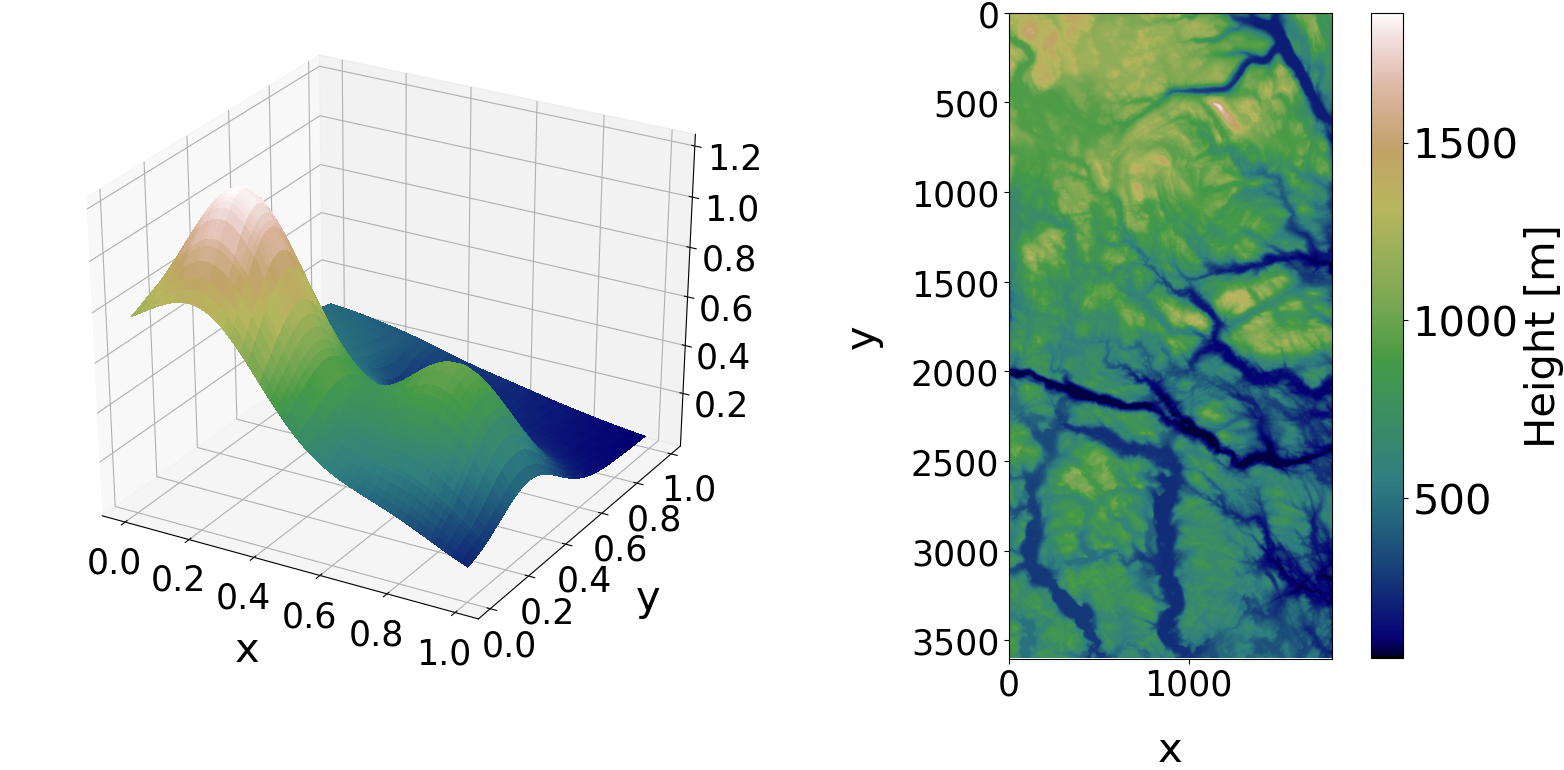
\includegraphics[width=\columnwidth]{Input_data.png}
  \caption{The Franke function (left) used for linear regression and a sample MNIST data (right) with the corresponding label used for classification.}
  \label{Input_data}
\end{figure}

Scaling of data sets is very effective for most of the ML algorithms. Thus, for our classification and linear regression problems, we have scaled respectively the MNIST data set and the design matrix of the regression problem by subtracting the mean and dividing with the standard deviation. 

\subsection{Error metrics}
We measure the performance of our regression and classification models using error metrics. For our classification problem we use the so-called accuracy score. The accuracy is the ratio of the number of correct predictions to the total number of input samples, that is
\begin{align}
    \text{Accuracy} = \frac{\sum_{i=1}^n I(t_i = y_i)}{n},
\end{align}
where $I$ is an indicator function giving a result of $1$ if $t_i = y_i$ otherwise $0$. Here $t_i$ represents the target and $y_i$ denotes our prediction and $n$ is simply the number of targets $t_i$. The accuracy score is a normalized metric with values between $0$ and $1$, where $1$ is the highest possible score while $0$ is the lowest. 

The other metric often used for measuring the performance of a ML
algorithm for classification problems is the confusion matrix. This metric is a matrix (table) and each row represents the instances of an actual class and each column represents the instances of a predicted class. The name confusion matrix reflects the fact that it makes it easy for us to see what kind of confusions occurs in our classification algorithms. The values of the confusion matrix will be incremented by one when making a prediction. In our coordinate system, the elements in the diagonal are the correctly classified ones, while the elements out of the diagonal are misclassified. 

The performance of the linear regression methods is measured using the MSE and R2-score. The MSE calculates the average of the squared error. The larger the value of the MSE the poorer the performance of the model. MSE is mathematically defined as
\begin{align}
    MSE = \frac{1}{n}
    \sum_{i=0}^{n-1}(y_i-\hat{y}_i)^2,
    \label{eq:MSE}
\end{align}
where $y_i$ is the actual data value, $\hat{y_i}$ is the predicted data point, and $n$ is the total number of data samples. Moreover, the $R^2$ score is a normalized error metric and its values vary between $0$ and $1$. $R^2$ represents the proportion of the variance in the dependent variable that is predictable from the independent variables. Mathematically, the $R^2$ score is given by
\begin{align}
    R^2 = 1 - \frac{\sum_{i=0}^{n - 1} (y_i - \hat{y}_i)^2}{\sum_{i=0}^{n - 1} (y_i - \bar{\mathbf{y}})^2}.
    \label{eq:R2}
\end{align}
where $\bar{\mathbf{y}}$ is the mean of $\mathbf{y}$. An $R^2$ score of $0$ means that the model is as accurate as the mean of the data and a negative score indicates that the mean is a better fit than the model.

\subsection{Implementation}
To perform linear regression, multinomial logistic regression, and NN-based regression and classification, we have used a fully object oriented python classes with a standard $\mathbf{NumPy}$ library for linear operations. For solving the linear regression problem, instead of using the analytical solutions \cite{Jing2020}, in this project we use the SGD method. A pseudo-code in algorithm \ref{alg-sgd} illustrates the steps followed to estimate the regression or classification parameters using the SGD method \cite{GoodBengCour16}. For the NNs, the gradients are computed using the back-propagation algorithm \cite{nielsenneural}.
\begin{algorithm}[H]
    \caption{Stochastic Gradient Descent (SGD) method}
    \label{alg-sgd}
    \begin{algorithmic}[1]
        \Require Learning rate $\eta$
        \Require Initial parameter $\mathbf{\theta}$
        \Require $\mathcal{N}_{epoch}$, $\mathcal{N}_{mbatch}$
        \For{i to $\mathcal{N}_{epoch}$}
            \State Sample a minibatch of $\mathcal{N}_{mbatch}$ examples from the training set $\{\mathbf{x}^{(1)},\mathbf{x}^{(2)},\dots,\mathbf{x}^{(\mathcal{N}_{mbatch})}\}$
            \State Set the gradient $\mathbf{g} = 0$
            \For{t to $\mathcal{N}_{mbatch}$}
            \State Compute gradient estimate: $\mathbf{g} = \mathbf{g} + \nabla \mathcal{C}(\theta_t)$
            \EndFor
            \State Apply update: $\mathbf{\theta} \leftarrow \mathbf{\theta} -\eta \mathbf{g}$ 
        \EndFor
    \end{algorithmic}
\end{algorithm}
To benchmark our implementation of the different regression and classification problems, we compare our results with the results from a $\mathbf{Scikit}$-$\mathbf{learn}$ library. Though, our results are slightly poor, we are highly encouraged by the consistency of our implementations compared to the two professional libraries. Furthermore, to complement our implementation, we use unit tests to allow us to test the individual units of our source code and determine whether they are fit for use.  

In this project, we have implemented three different ways of using the learning rate in the SGD algorithm. These three options of the learning rates include: (i) fixed, (ii) linearly decaying, and (iii) exponentially decaying. Figure \ref{exp_eta} shows these learning rates as a function of the number of epochs.

\begin{figure}[H]
  \centering
  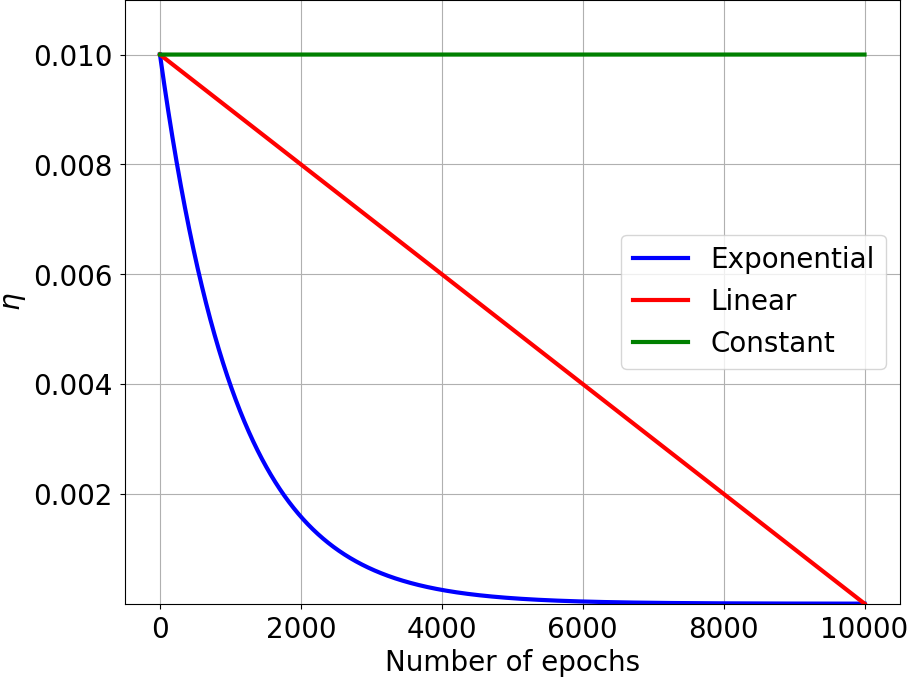
\includegraphics[width=4in,keepaspectratio]{Project2/exp_eta.png}
  \caption{Three different ways of varying the learning rate $\eta$ in SGD as a function of the number of epochs.}
    \label{exp_eta}
\end{figure}

\section{Results}
In this section we present the results of our analysis for the linear regression, multi-class regression and the use of NNs for regression and classification problems. We make a thorough analysis of the SGD algorithm for solving linear regression problems and compare the results with the NN-based methods. Finally, we use multinomial logistic regression and NN-based method for classifying handwritten digits from the MNIST dataset.

\subsection{Linear regression using SGD}
We start our analysis of linear regression on the noisy Franke function dataset by considering the Ordinary Least Squared (OLS) method with the SGD algorithm. Here, we first tune the learning rate parameter. The learning rate in ML applications is often considered the single most important hyperparameter that needs to be tuned at the beginning \cite{Bengio2012}. Using the fact that linear regression problems have analytical gradients, we have chosen to tune the learning rate using the GD algorithm. Figure \ref{LinearReg_CV_eta_GD} show the MSE (cost function) as a function of the number of gradient descent iterations for three different learning rates. We have selected the largest learning rate using the fact that the GD algorithm converges only when $\eta<2/\lambda_{max}$, where $\lambda_{max}$ is the maximum eigenvalue of the Hessian matrix \cite{Pankaj}. Thus, for $\eta=0.0382$, the MSE is the smallest for all the iterations, but the MSE for $\eta=0.01$ reaches the same value when the number of iterations are $\sim 10^{4}$ (see Figure \ref{LinearReg_CV_eta_GD}). Therefore, for our analysis of the linear regression with the SGD method, we have chosen $\eta=0.01$ to be our initial learning rate.

\begin{figure}[H]
  \centering
  \includegraphics[width=\columnwidth]{Project2/LinearReg_CV_eta_GD.png}
  \caption{The MSE (linear regression cost function) as a function of the number of gradient descent iterations for three different learning rates. Notice, both the vertical and horizontal axis are in logarithmic scales.}
    \label{LinearReg_CV_eta_GD}
\end{figure}

The number of epochs and the mini-batch size of a SGD method needs to be optimized for a successful application of the method in solving the linear regression problem. To assess such a performance, we use the test MSE and $R^2$-score metrics and perform a gird search on the number of epochs and the mini-batch sizes (cf. Figure \ref{LinearReg_CV_const_eta_SGD}). To obtain a statistically stable result and reduce the fluctuations, which is inherent in the SGD algorithm, we apply a $5$-fold cross validation to our analysis. Consequently, the optimal number of epochs and the mini-batch size for our OLS regression is found to be $5000$ and $300$, respectively. However, we have performed the same analysis with a linearly and exponentially decaying learning rate, but observe that a linear decay resulted in the smallest MSE and highest $R^2$-score (cf. Figure \ref{LinearReg_CV_linear_eta_SGD}). 

\begin{figure}[H]
  \centering
  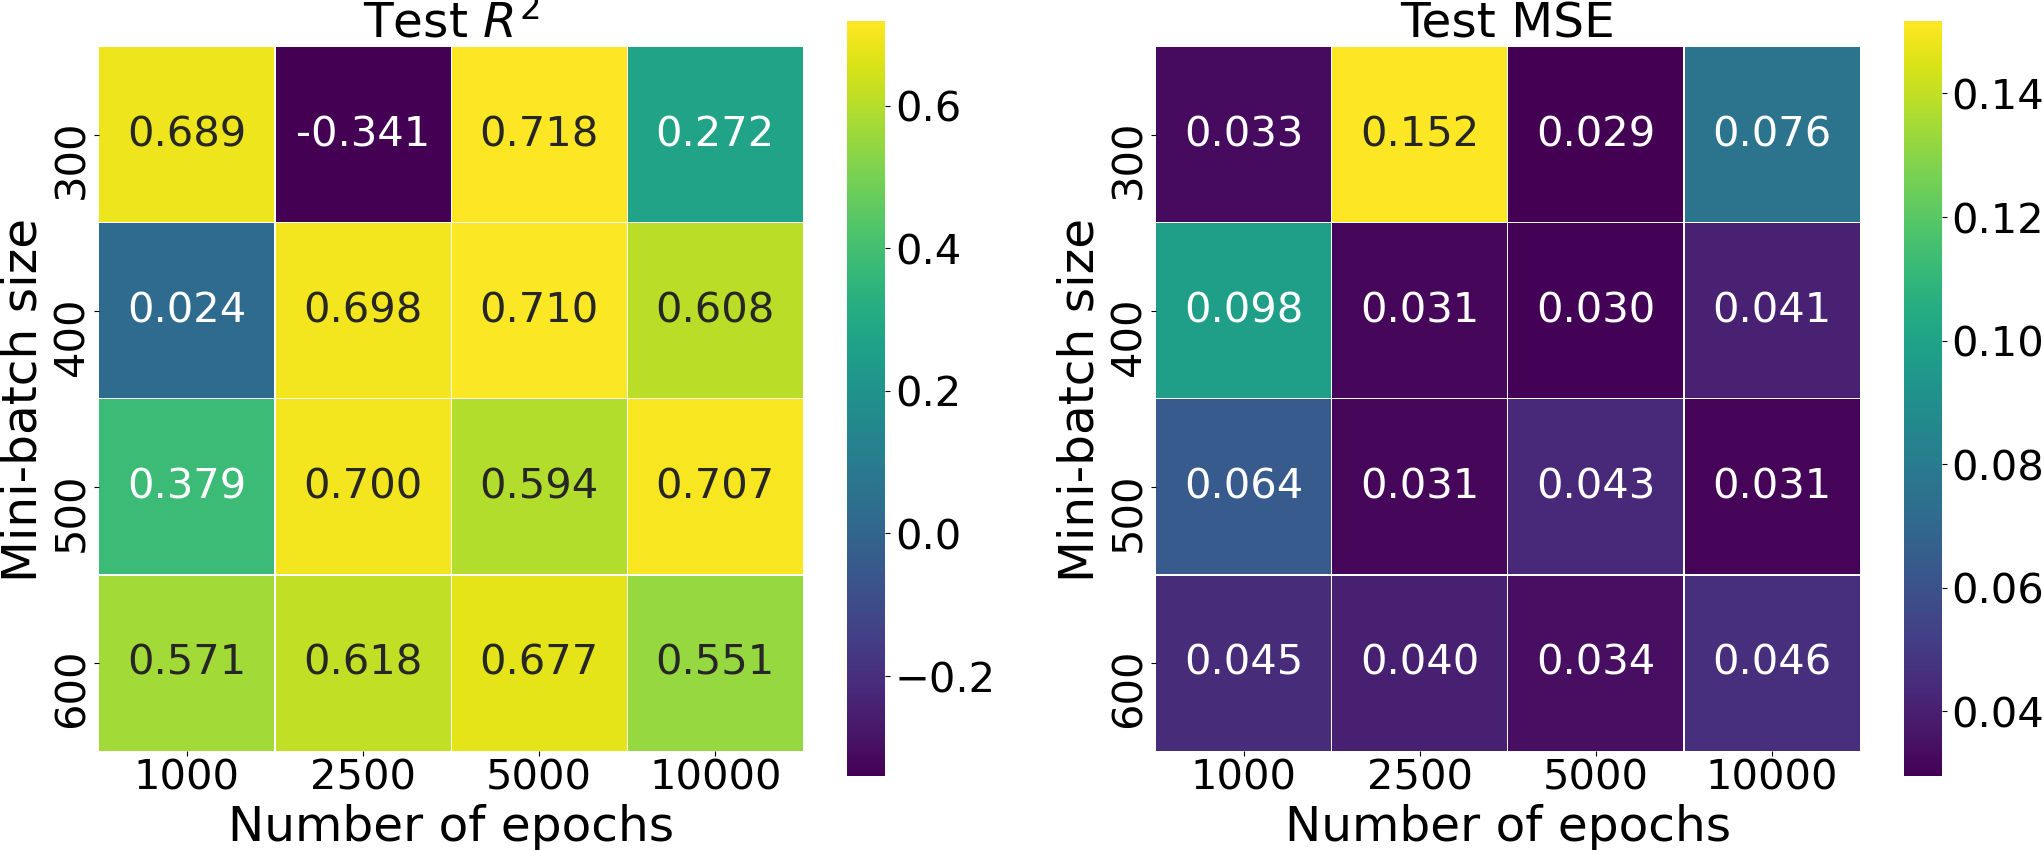
\includegraphics[width=\columnwidth]{Project2/LinearReg_CV_const_eta_SGD.png}
  \caption{The test $R^2$-score (left) and MSE (right) for a grid search of the number of epochs and the mini-batch size. Here, the learning rate is fixed to $0.01$ and a $5$-fold cross validation is used.}
    \label{LinearReg_CV_const_eta_SGD}
\end{figure}

\begin{figure}[H]
  \centering
  \includegraphics[width=\columnwidth]{Project2/LinearReg_CV_linear_eta_SGD.png}
  \caption{The test $R^2$-score (left) and MSE (right) for a grid search of the number of epochs and the mini-batch size. Here, the learning rate is linearly decaying from an initial value of $0.01$ to a final value of $10^{-6}$ and a $5$-fold cross validation has been used.}
    \label{LinearReg_CV_linear_eta_SGD}
\end{figure}

So far we have fitted and predicted the noisy Franke function using a $5^{th}$-order polynomial function and the OLS method with the SGD algorithm. However, the OLS method is notorious for suffering from overfitting problem. To overcome such a problem often the first choice is to apply regularization methods. Here, we have chosen to use Ridge regression and determine its corresponding learning rate and the penalty (regularization) hyperparameter using a grid search with a $5$-fold cross validation (see Figure \ref{LinearReg_CV_linear_eta_lamb_SGD}). When applying the grid search, we have set the number of epochs to $10^4$, the mini-batch size to $300$, and we have allowed the learning rate to decay linearly. Comparing the result of the OLS and Ridge regressions, we can observe that both methods performed similarly. This is not surprising because fitting a $5^{th}$-order polynomial function to the Franke function dataset with only $10\%$ added noise does not result in overfitting.

\begin{figure}[H]
  \centering
  \includegraphics[width=\columnwidth]{Project2/LinearReg_CV_linear_eta_lamb_SGD.png}
  \caption{The test $R^2$-score (left) and MSE (right) for a grid search of the learning rate $\eta$ and the penalty parameter $\lambda$ of Ridge regression. Notice, the learning rate is linearly decaying as a function of the number of epochs and a $5$-fold cross validation has been used.}
    \label{LinearReg_CV_linear_eta_lamb_SGD}
\end{figure}

Finally, the different methods of solving the linear regression problem are compared and the results are summarized in Table \ref{linreg}. Here, we refer to the analytical inversion method \cite{Jing2020} of solving linear regression problems as simply Analytical. From Table \ref{linreg} we can see that the performance of the OLS and Ridge (with $\lambda=10^{-3}$) regression are equivalent. It is also possible to observe that the SGD algorithm is slightly poor compared to the analytical inversion based method.

\begin{table}[ht]
\begin{center}
  \begin{tabular}{| l | l | l |}
  \hline
    Method &  Test MSE & Test $R^2$-score \\[0.10cm]\hline\hline
     & &  \\
     SGD [OLS] & $0.020$ & $0.743$ \\[0.10cm]
    SGD [Ridge] & $0.021$ & $0.742$\\[0.10cm]
     Analytical [OLS] & $0.018$& $0.777$\\[0.10cm]
     Analytical [Ridge] & $0.017$& $0.790$\\[0.10cm]
     \hline
  \end{tabular}
\end{center}
\caption{The performance comparison of the different methods of solving the linear regression problem.}
\label{linreg}
\end{table}

\subsection{Regression using neural networks} 
NNs are an extension to MLPs (cf. section \ref{sec-nn}). In this project we have used the most basic NN architecture, a fully connected NN. For solving regression problems using NNs, we use the MSE as a cost function where the predicted value is compared to the ground truth label and averaged over the all the predictions. Moreover, for solving a regression problem, we set the output layer to have a single node, and the corresponding activation function to be an identity function, where their is no non-linearity.

To perform regression on the noisy Franke function, We have chosen a fully connected NN with only two hidden layers where each having $20$ nodes (neurons). The learning rate and the regularization hyperparameter have been tuned by using a grid search with a $5$-fold cross validation. Figure \ref{LinearReg_CV_eta_lamb_NN} shows the test MSE and $R^2$-score when using the sigmoid function as an activation function for both the two hidden layers. In addition, for estimating the weights and bias parameters, we have used the SGD algorithm with $1000$ number of epochs and a mini-batch size of $32$. The weights were initialized using using a normal distribution while we have used a small constant number $0.01$ to initialize the biases. For such a NN it is possible to observe that regularizing the regression produced a poor result compared to its corresponding result without regularization. Figures \ref{LinearReg_CV_eta_lamb_NN_relu} and \ref{LinearReg_CV_eta_lamb_NN_elu} show the grid search with $5$-fold cross validation to find the optimal learning rate and regularization hyperparameters of the NN with ReLU and Leaky ReLU as activation functions, respectively. Therefore, for our simple NN with only two hidden layers, the best performance for solving the regression problem is achieved by using the Leaky ReLU as an activation function and using a regularization hyperparameter of $\lambda=10^{-4}$.

\begin{figure}[H]
  \centering
  \includegraphics[width=\columnwidth]{Project2/LinearReg_CV_eta_lamb_NN_sigmid.png}
  \caption{The test $R^2$-score (left) and MSE (right) for a grid search with $5$-fold cross validation of the learning rate $\eta$ and the regularization parameter $\lambda$ when using the sigmoid function as the activation function of the hidden layers.}
  %{The Franke function (left) used for linear regression and a sample MNIST data (right) with the corresponding label used for classification.}
    \label{LinearReg_CV_eta_lamb_NN}
\end{figure}

\begin{figure}[H]
  \centering
  \includegraphics[width=\columnwidth]{Project2/LinearReg_CV_eta_lamb_NN_relu.png}
  \caption{The test $R^2$-score (left) and MSE (right) for a grid search with $5$-fold cross validation of the learning rate $\eta$ and the regularization parameter $\lambda$ when using the ReLU function as the activation function of the hidden layers.}
  %{The Franke function (left) used for linear regression and a sample MNIST data (right) with the corresponding label used for classification.}
    \label{LinearReg_CV_eta_lamb_NN_relu}
\end{figure}

\begin{figure}[H]
  \centering
  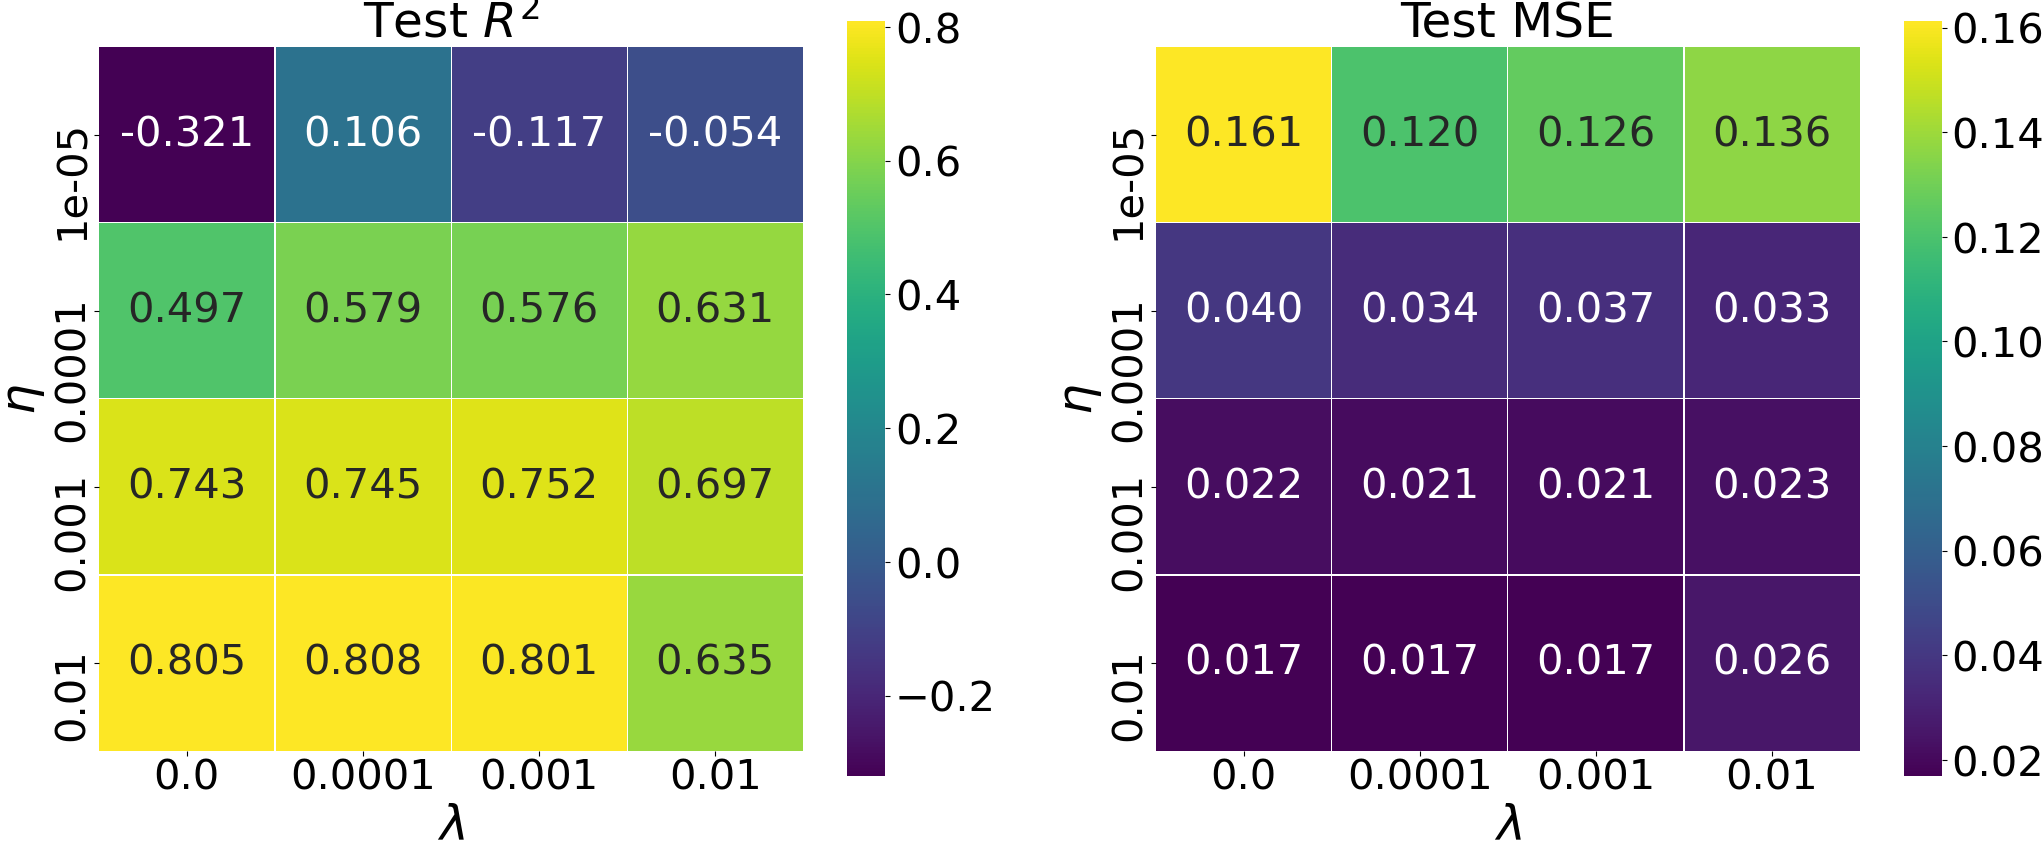
\includegraphics[width=\columnwidth]{Project2/LinearReg_CV_eta_lamb_NN_elu.png}
  \caption{The test $R^2$-score (left) and MSE (right) for a grid search with $5$-fold cross validation of the learning rate $\eta$ and the regularization parameter $\lambda$ when using the Leaky ReLU function as the activation function of the hidden layers.}
  %{The Franke function (left) used for linear regression and a sample MNIST data (right) with the corresponding label used for classification.}
    \label{LinearReg_CV_eta_lamb_NN_elu}
\end{figure}

Finally, we have compared the performance of our implementation of the NNs for solving a regression problem with that of $\mathbf{Scikit}$-$\mathbf{learn}$ library's $\texttt{MLPRegressor}$. All the methods in Table \ref{regNN} have been analysed using the same parameters (i.e., two hidden layers with $20$ neurons each, $\lambda=10^{-4},\eta=0.01$, number of epochs $=10^3$, and mini-batch size $=32$) except we have used Leaky ReLU and ReLU activation functions in our implementation and $\mathbf{Scikit}$-$\mathbf{learn}$, respectively. From Table \ref{regNN} we can observe that our implementation of the NNs managed to perform quite good, but slightly poor compared to $\mathbf{Scikit}$-$\mathbf{learn}$ library's result.

\begin{table}[H]
\begin{center}
  \begin{tabular}{| l | l | l |}
  \hline
    Method &  Test MSE & Test $R^2$-score \\[0.10cm]\hline\hline
     & &  \\
    Our NN & $0.024$ & $0.692$ \\[0.10cm]
    Scikit-learn & $0.013$ & $0.841$\\[0.10cm]
     \hline
  \end{tabular}
\end{center}
\caption{The performance comparison of our implementation of the NNs method and the $\mathbf{Scikit}$-$\mathbf{learn}$ library for solving a regression problem.}
\label{regNN}
\end{table}

\subsection{Classification}
The classification task we consider in this project is that of identifying handwritten digits using the MNIST dataset \cite{lecun-mnisthandwrittendigit-2010}. Randomly selected training data sets with their corresponding outputs (labels) are shown in Figure \ref{Digits_data}. To perform such a multi-class classification using both NN and multinomial logistic regression requires the so called softmax function, which can be thought of as a statistical model which assigns a probability that a given input image corresponds to any of the $10$ handwritten digits. In this section, we first classify the handwritten digits using a multi-class (multinomial) logistic regression (also called softmax regression), and then we will apply NNs and quantitatively compare the results of two methods with the corresponding $\mathbf{Scikit}$-$\mathbf{learn}$ library results. 

\begin{figure}[H]
  \centering
  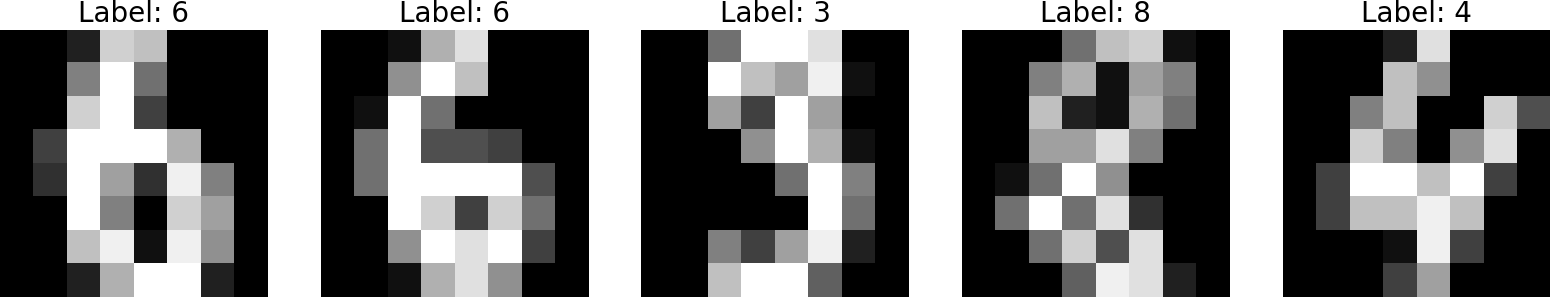
\includegraphics[width=\columnwidth]{Project2/Digits_data.png}
  \caption{Samples of the MNIST training data sets with their corresponding labels.}
    \label{Digits_data}
\end{figure}

\subsubsection{Classification using multinomial logistic regression}
Unlike linear regression, the multinomial logistic regression cost function (see Equation \ref{mclog-cost}) is non-linear and hence does not have analytical (closed form) solution. Here, we have used the SGD algorithm to find the optimal weights and biases. Figure \ref{Digits_CV_Loss} show the minimization of the negative logarithmic loss function (see Equation \ref{mclog-cost}) using the SGD algorithm with $10^4$ number of epochs and a mini-batch size of $32$. However, such an optimization algorithm also have extra parameters (e.g., $\eta$ and $\lambda$) that needs to be tuned before applying it to train our dataset.

\begin{figure}[H]
  \centering
  \includegraphics[width=\columnwidth]{Project2/Digits_CV_Loss.png}
  \caption{The minimization of the multinomial logistic regression cost function using the SGD algorithm.}
  %{The minimization of the multi-class regression cost function using a SGD algorithm.}
    \label{Digits_CV_Loss}
\end{figure}

We have tuned the learning rate and the regularization hyperparameter $\lambda$ of the SGD algorithm using a grid search with $5$-fold cross validation  (cf. Figure \ref{LogReg_CV_eta_lmb_SGD}). Notice, the case where $\lambda=0$ corresponds to the absence of regularization. Based on the test accuracy score, we can observe that the most optimal parameters are $\eta=0.1$ and $\lambda=0.01$.

\begin{figure}[H]
  \centering
  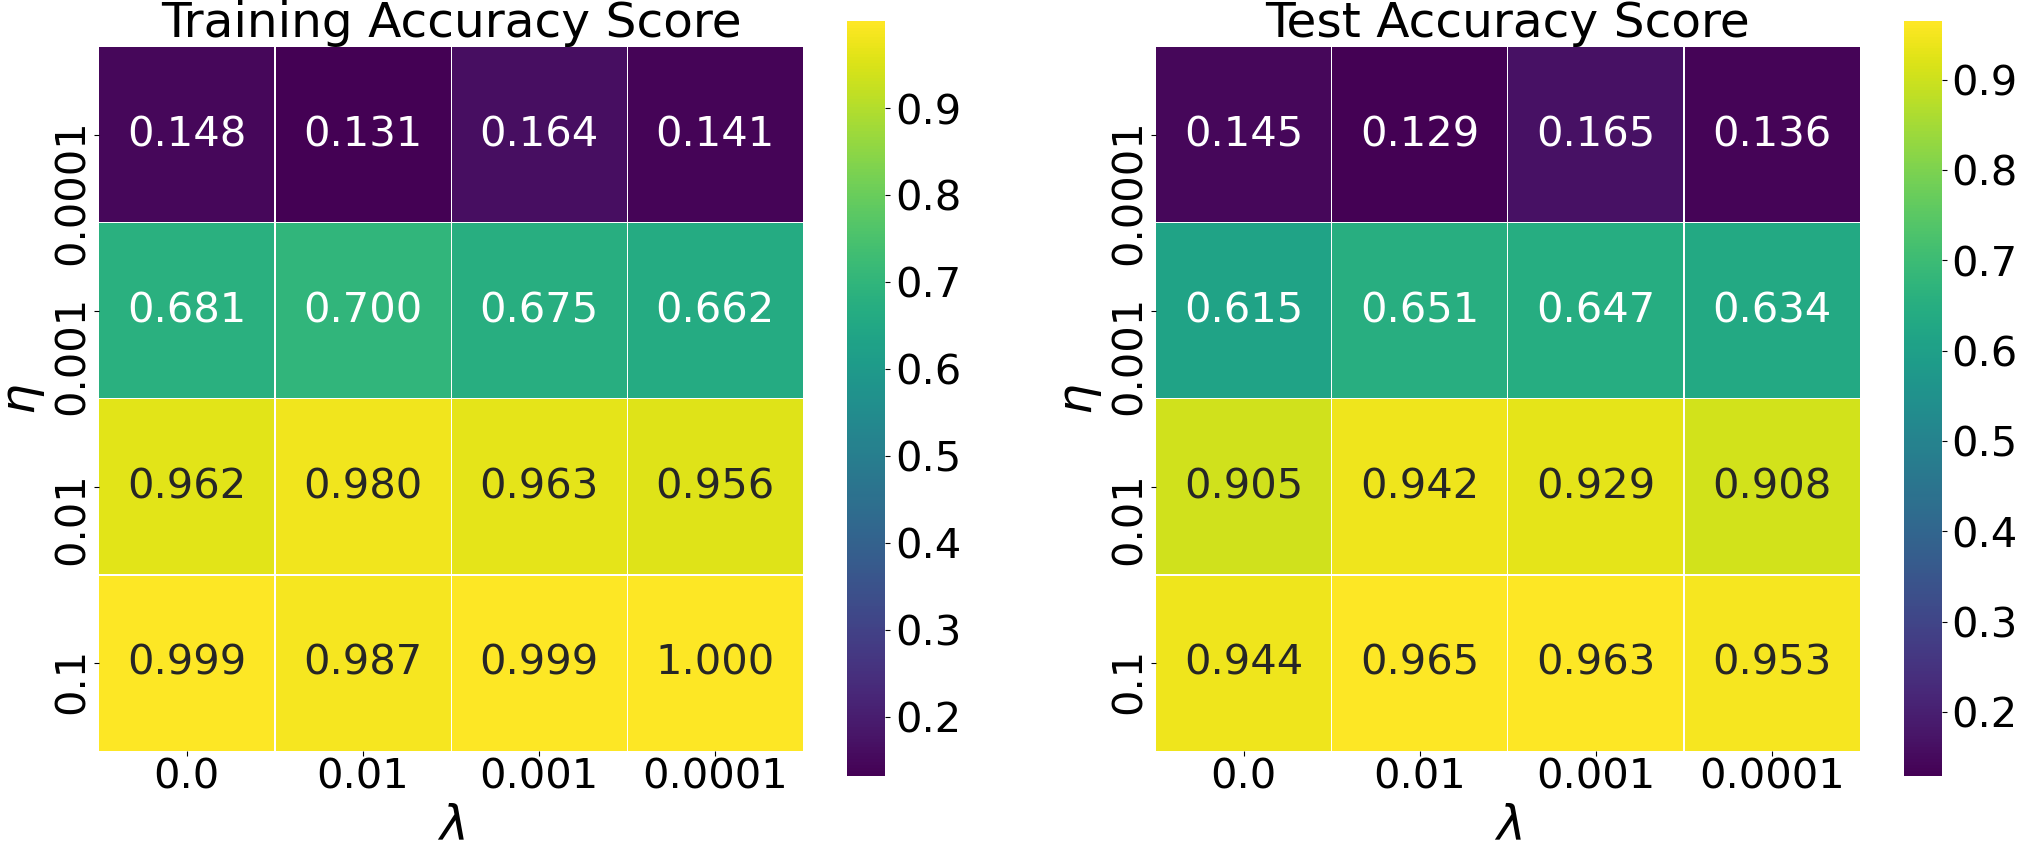
\includegraphics[width=\columnwidth]{Project2/LogReg_CV_eta_lmb_SGD.png}
  \caption{The learning rate $\eta$ and regularization hyperparameter $\lambda$ grid search for training (left) and test (right) data sets. The accuracy score has been used as the metric.}
    \label{LogReg_CV_eta_lmb_SGD}
\end{figure}

To compare the performance or our multinomial logistic regression with that of $\mathbf{Scikit}$-$\mathbf{learn}$ in classifying the MNIST dataset, we have selected the confusion matrix our metric. Figure \ref{Digits_confusionM} shows the performance of our multinomial logistic regression, which is comparable to $\mathbf{Scikit}$-$\mathbf{learn}$'s $\mathbf{LogisticRegression}$. Moreover, we can observe that the classification capability of the multinomial logistic regression is excellent.

\begin{figure}[H]
  \centering
  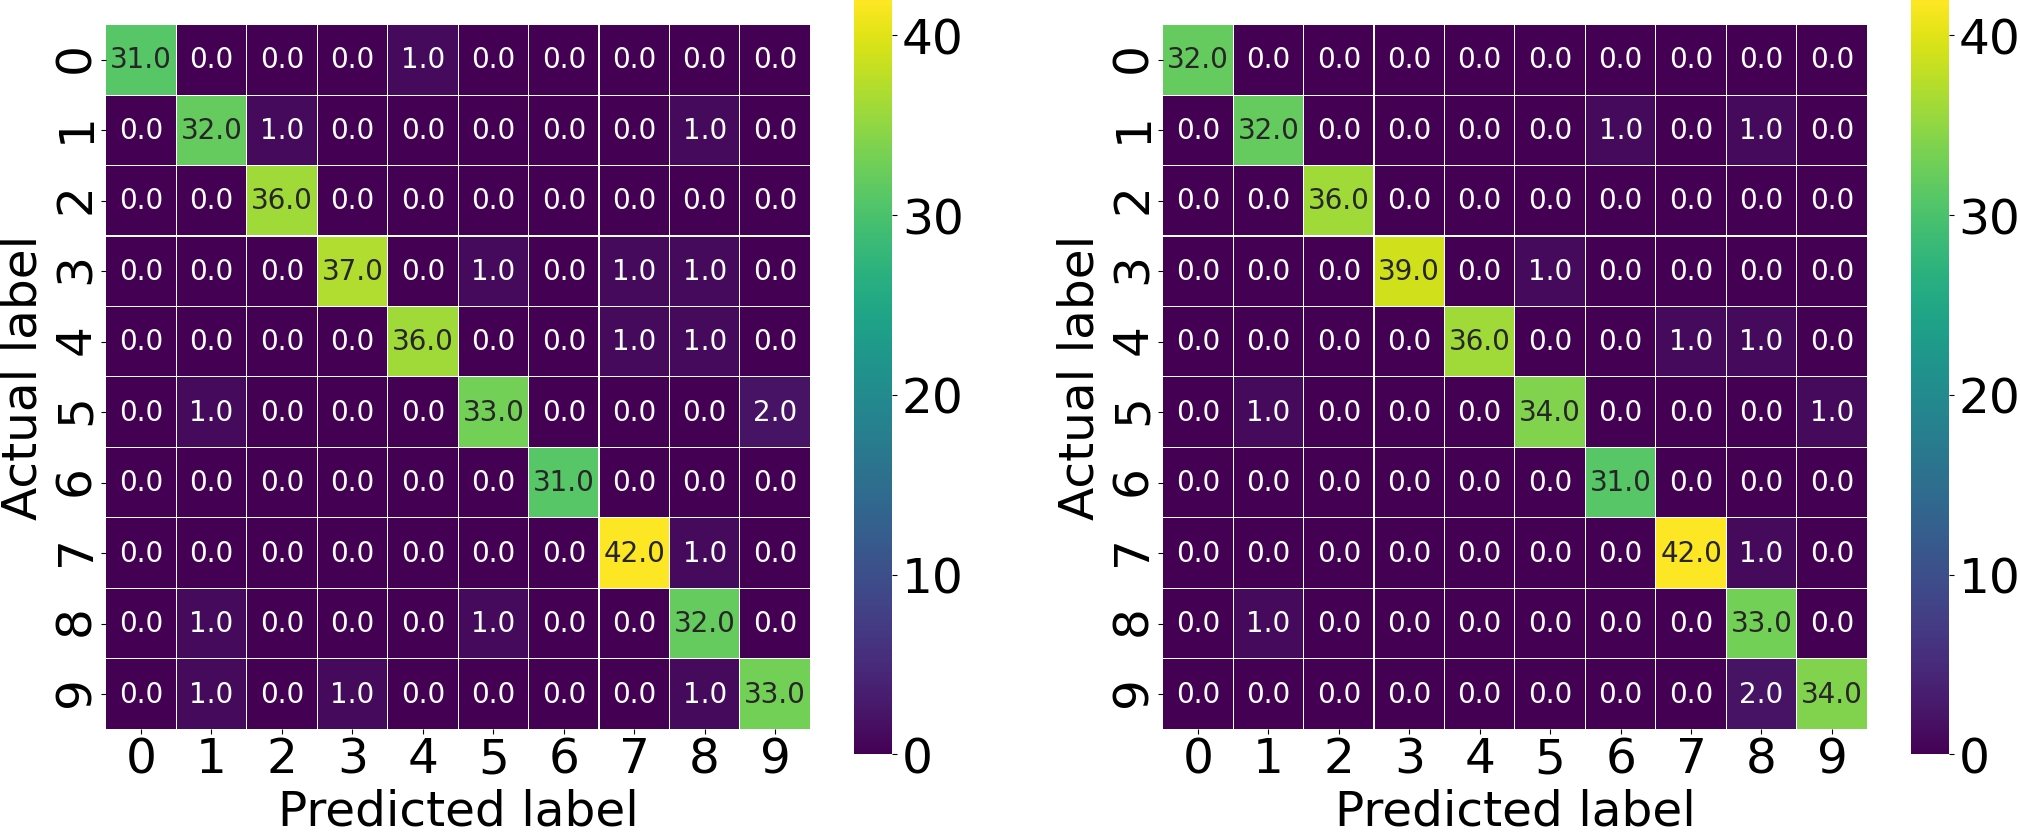
\includegraphics[width=\columnwidth]{Project2/Digits_confusionM.png}
  \caption{The confusion matrix and the test accuracy score of our code (left) and that of $\mathbf{Scikit}$-$\mathbf{learn}$ (right). All results have been obtained after a $5$-fold cross validation.}
    \label{Digits_confusionM}
\end{figure}

\subsubsection{Neural networks for classification}
We now classify the handwritten digits in the MNIST dataset using fully connected NNs. The parameters of the network are the following: single-hidden-layer, $50$ neurons in the hidden layer, $1000$ number of epochs, and mini-batch size of $100$. The optimal learning rate and the regularization hyperparameter $\lambda$ have been determined using a grid search with $5$-fold cross validation and accuracy score as the error metric. The result of the grid search is shown in Figure \ref{NN_class_CV_eta_lmb}. Therefore, we have selected an optimal learning rate of $\eta=0.1$ and regularization hyperparameter of $\lambda=0.01$.

\begin{figure}[H]
  \centering
  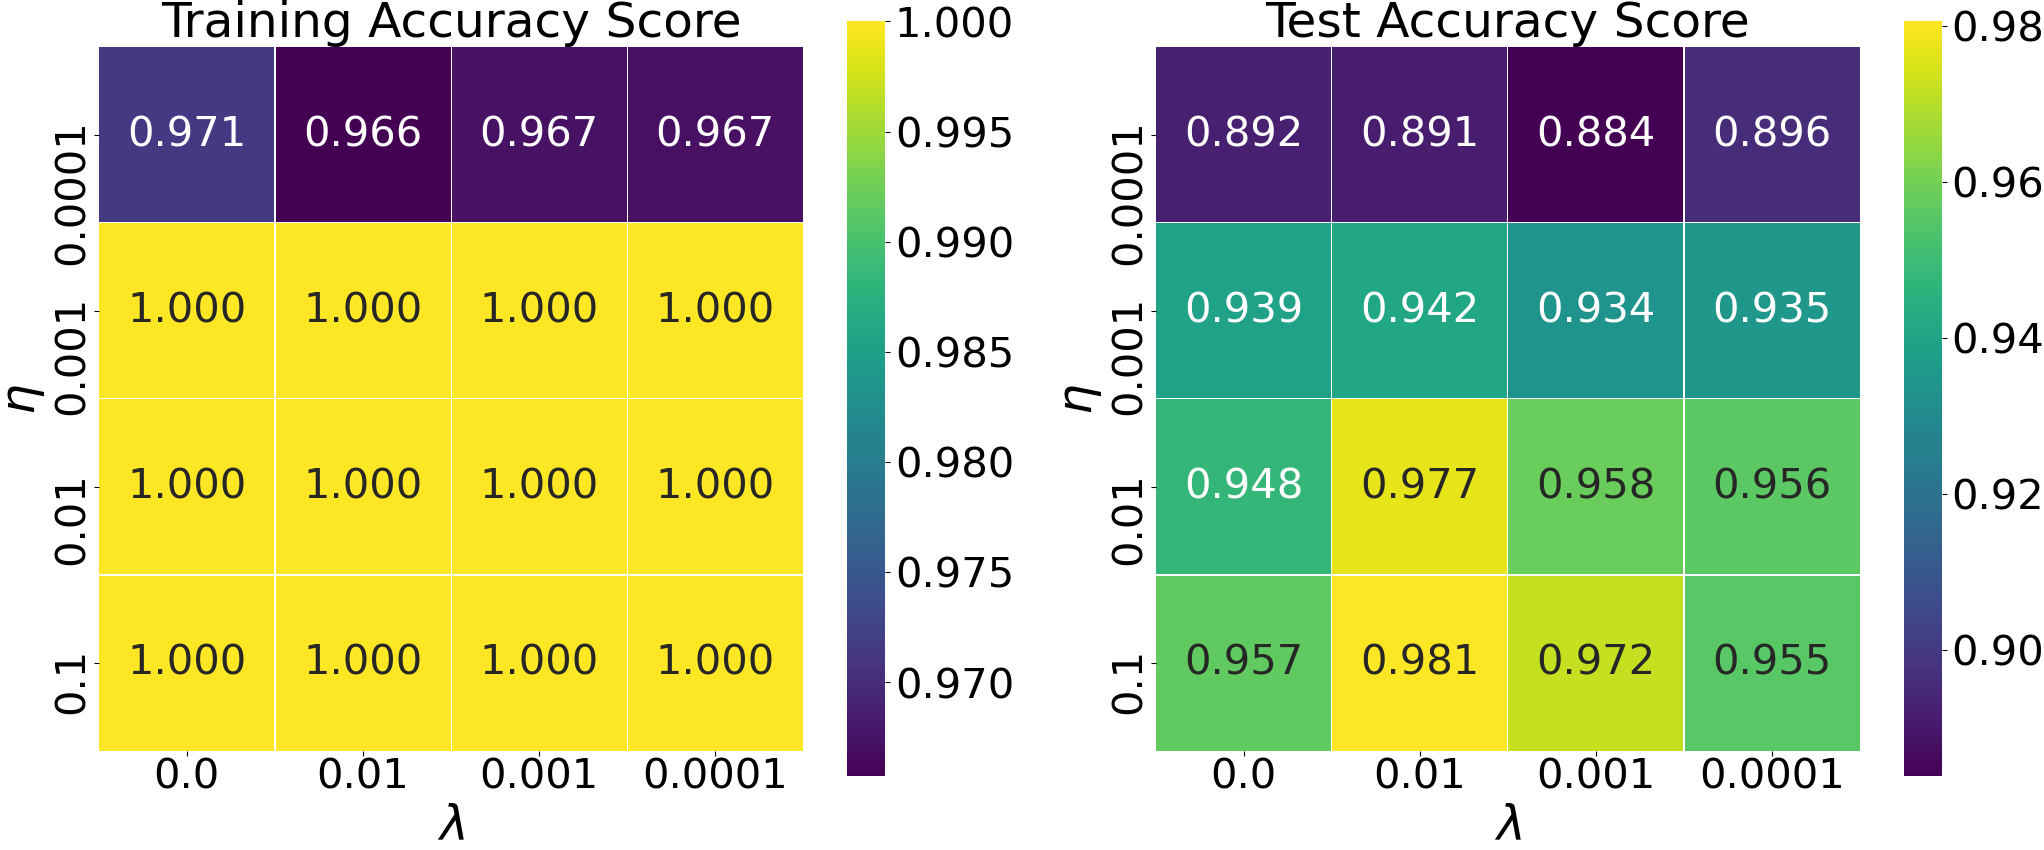
\includegraphics[width=\columnwidth]{Project2/NN_class_CV_eta_lmb.png}
  \caption{The learning rate $\eta$ and regularization hyperparameter $\lambda$ grid search for training (left) and test (right) data sets. The accuracy score has been used as the metric.}
    \label{NN_class_CV_eta_lmb}
\end{figure}

To benchmark our implementation of the NNs, we compare the results from our code with that of $\mathbf{Scikit}$-$\mathbf{learn}$ (see Figure \ref{NN_Digits_confusionM}) using the confusion matrix as our quantitative metric. The performance of the two NNs are comparable, but the result of $\mathbf{Scikit}$-$\mathbf{learn}$ is slightly better.

\begin{figure}[H]
  \centering
  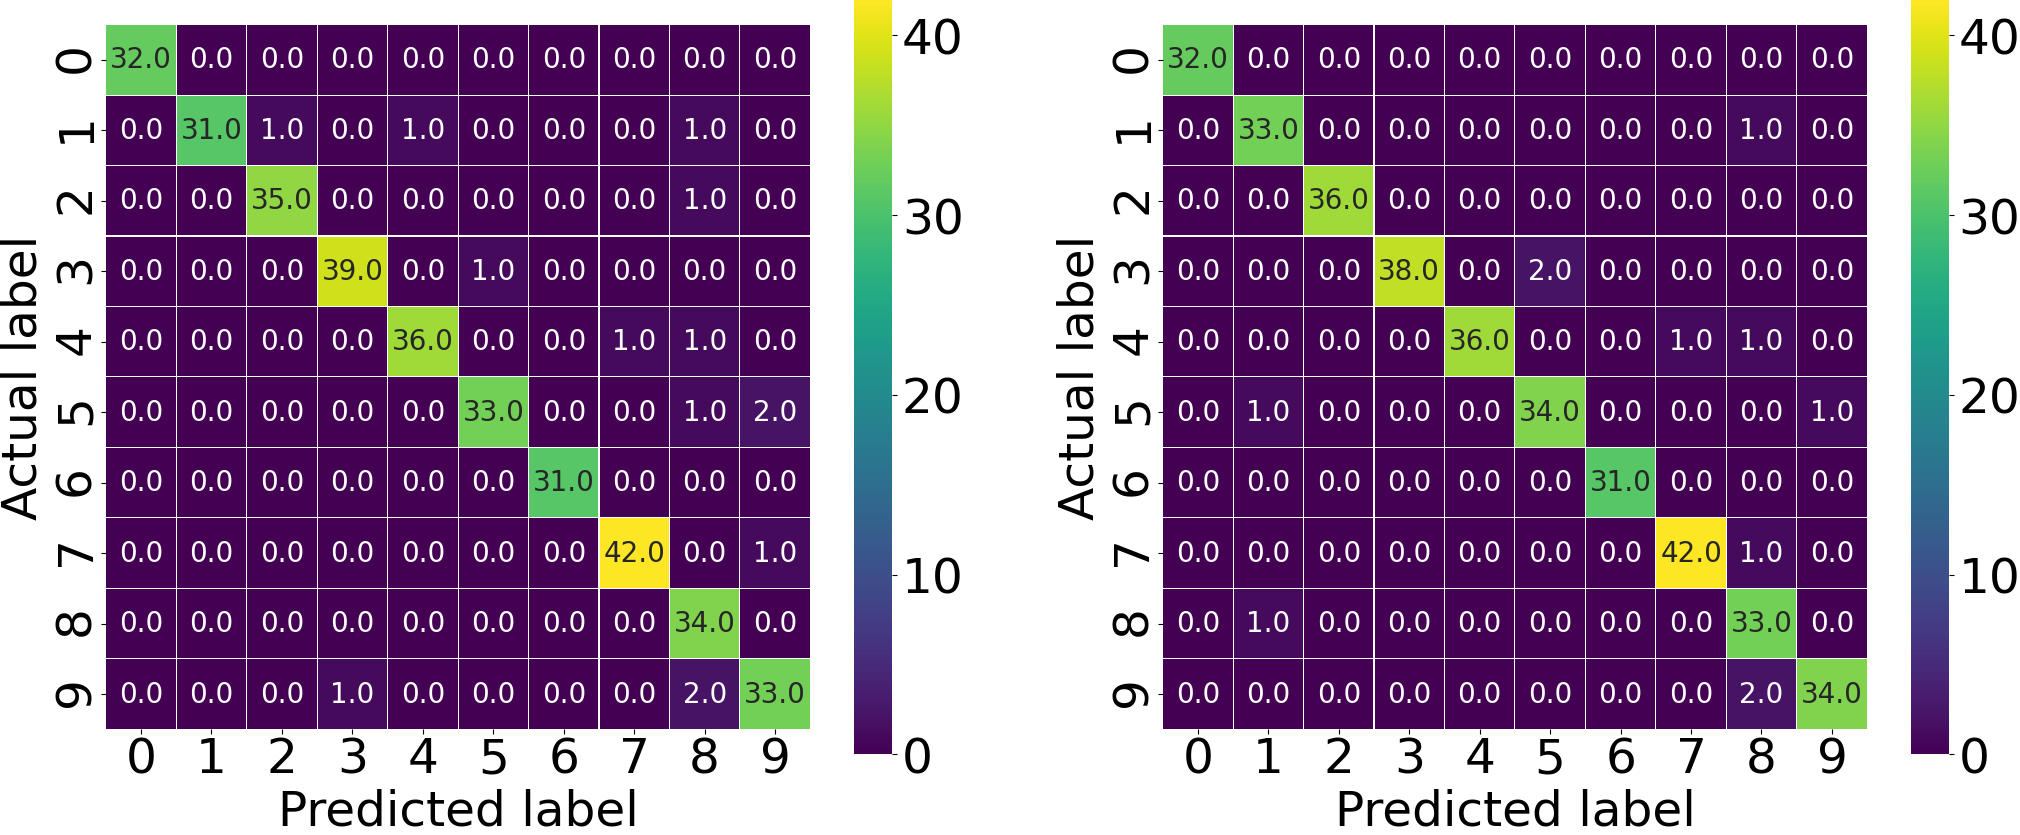
\includegraphics[width=\columnwidth]{Project2/NN_Digits_confusionM.png}
  \caption{The confusion matrix and the test accuracy score of our code (left) and that of $\mathbf{Scikit}$-$\mathbf{learn}$ (right). All results have been obtained after a $5$-fold cross validation.}
    \label{NN_Digits_confusionM}
\end{figure}

Finally, comparing the performance of NNs with the multinomial logistic regression for classifying the MNIST dataset, we have observed that NNs are slightly better than the multinomial logistic regression (cf. Table \ref{classNN}). This is might be due to the fact that the latter is a linear classifier while the first is a non-linear classifier.

\begin{table}[H]
\begin{center}
  \begin{tabular}{| l | l | l |}
  \hline
    Classification method &  Test accuracy score & Training accuracy score \\[0.10cm]\hline\hline
     & &  \\
    Our NN & $0.961$ & $1.0$ \\[0.10cm]
    Scikit-learn NN & $0.969$ & $1.0$\\[0.10cm]
    Our softmax reg. & $0.958$ & $0.986$ \\[0.10cm]
    Scikit-learn softmax reg. & $0.969$ & $0.999$\\[0.10cm]
     \hline
  \end{tabular}
\end{center}
\caption{The performance comparison of our implementation of the NNs and multinomial regression methods with the corresponding  $\mathbf{Scikit}$-$\mathbf{learn}$ library for solving a classification problem.}
\label{classNN}
\end{table}

\section{Discussion}
Linear regression is a great test case for the GD methods. This is mainly due to the following desirable properties: (i) has an analytical solution, (ii) the gradient can be computed analytically, and (iii) the cost function is convex which guarantees that gradient descent converges for small enough learning rates. Moreover, the SGD method inherits the advantages of the GD method and in addition provides a computationally faster method and unlike the GD method avoids getting stuck in the local minimum.  When performing SGD-based linear regression we have encountered an overflow error, when the mini-batch size is reduced below $300$. We could not find the root cause of this problem in our implementation. Therefore, we have only tested mini-batch sizes larger than $300$.

The performance of the SGD algorithm is highly dependant on its parameters, especially the learning rate. Most of the strategies proposed for choosing this parameter does not have theoretical guarantees, whereas those backed by theories often do not shine in practice. In this project, we have studied heuristic step size schedules that are constant, linearly decaying, and exponentially decaying per epochs. Using a $5$-fold cross validation test, we have found that the linearly decaying step size schedule gave the best result.

Finding the optimal hyperparameters using a grid search with cross validation is computationally expensive and thus allowed us only to explore a small portion of the hyperparameter space. Nevertheless, one might use a random search to find the optimal hyperparameters and consequently obtain a better model for regression and classification.

The application of NNs for classification problems have resulted in a better performance compared to multinomial logistic regression methods. However, NNs have much more hyperparameters, which gives them higher flexibility. Here, it is crucial to notice that when tuning hyperparameters, we need to use cross validation.

\section{Conclusion}
We analyse the performance of linear regressors and NNs for solving a regression problem. We have also analysed multinomial logistic regressors and fully connected NNs for classification problems. All the methods are benchmarked by comparing with the $\mathbf{Scikit}$-$\mathbf{learn}$ library. For the regression problem on the noisy Franke function data, we find the two-hidden-layer NN performs slightly worse than the SGD-based OLS and Ridge regression methods. Moreover, our implementation of NNs for regression results in a test MSE of $0.024$ and $R^2$-score of $0.692$, while the corresponding result with $\mathbf{Scikit}$-$\mathbf{learn}$ are MSE of $0.013$ and $R^2$-score of $0.841$. For the classification problem of identifying the handwritten digits from the MNIST dataset, the NNs performs better than multinomial logistic regressors. For a single-hidden-layer NN, we have found a test accuracy score of $0.961$ using our code and $0.969$ using that of $\mathbf{Scikit}$-$\mathbf{learn}$ library. The corresponding multinomial logistic regressors result are $0.958$ and $0.969$, respectively, using our code and $\mathbf{Scikit}$-$\mathbf{learn}$.

To avoid overfitting we have used regularization, but this method can be computationally expensive. Another way to avoid overfitting is by using early stopping. Though, we have not used it in this project, we think it is an elegant way of avoiding overfitting and suggest it as a future work. Moreover, we also would like to investigate the generalization capabilities of NNs for regression by creating test data sets outside the range of the training dataset.

\section{Acknowledgements}
We would like to thank Professor Morten Hjorth-Jensen and the teaching assistants in the course FYS-STK-4155/3155 for the many helps we got during this project.

%\bibliographystyle{plain}
%\bibliographystyle{siam}
\bibliography{sample}
\bibliographystyle{IEEEtran}

\end{document}
